\section{HLASM context tables}

HLASM context tables (in code referred simply as hlasm context) is composition of tables and stacks that describe state of the currently processed open-code (see \cref{fig06:hlasm}). This structure is persistent between source files within an open-code. It is created in analyzer and has the same lifespan. 

It is composed of:

\begin{itemize}
	\item \emph{Macro \& Copy storage} -- stores macro and copy definition definitions.
	\item \emph{ID storage} -- stores symbol identifiers.
	\item \emph{Scope stack} -- stores nested macro invocations and local variable symbols.
	\item \emph{Global variable symbol storage} -- stores global variable symbols.
	\item \emph{Source stack} -- stores nested source files.
	\item \emph{Processing stack} -- stores stack of processings in a source file.
	\item \emph{LSP context}
	\item \emph{Ordinary assembly context} -- encapsulates structures describing Ordinary assembly.
\end{itemize}

\begin{figure}
	\centering
	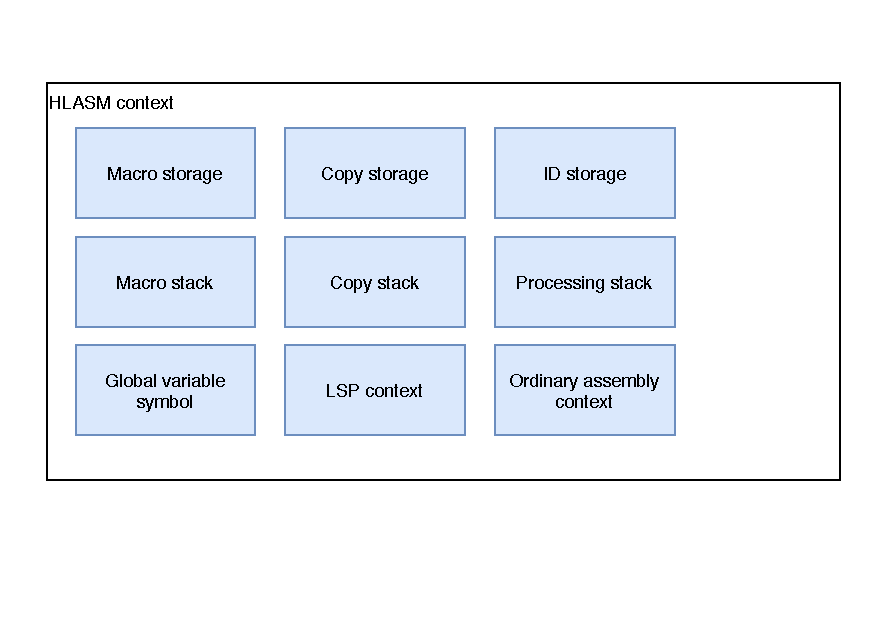
\includegraphics[width=\textwidth / 2]{img/hlasm_arch}
	\caption{The composition of HLASM context tables component}
	\label{fig06:hlasm}
\end{figure}

\subsection{Macros}

HLASM context stores visited macro definitions in the \emph{macro strorage}. 

Macro definition is represented by:
\begin{enumerate}
	\item \emph{Macro identifier}. It identifies the macro.
	\item \emph{Calling parameters}. They are assigned real value when the macro is called.
	\item \emph{Block of statement}. It represents the body of the macro.
	\item \emph{Block of copy nestings}. It is array with one-to-one relation with block of statements. Each entry is a list of in-file locations that represents how much was the statement nested in COPY calls.
	\item \emph{Label storage}. The storage of sequence symbol that occur in the macro definition.
\end{enumerate}

When macro is called, \emph{macro invocation} object is created. It shares the content of a respective macro definition with an exception of calling parameters as they are assigned real value passed with the call. Also, it contains index to the top statement of the invocation.

The macro invocation is stored in the context's \emph{scope stack}.

\subsection{Scope stack}

This stack holds information about the scope of variable symbols (see \cref{lab06:var_sym}). The scope changes when macro is visited. The initial scope is the open-code. 


The stack contains:
\begin{itemize}
	\item In-scope variable symbols.
	\item In-scope sequence symbols.
	\item Pointer to the macro invocation (NULL if in open-code).
	\item Branch counter (for ACTR instruction).
\end{itemize}

\subsection{COPY}

HLASM context stores visited COPY members in the \emph{copy strorage}.

COPY member definition is much more simple than the macro definition as it does not hold any more semantic information than the sequence of statements (the definition itself).

When copy is visited, copy member invocation is created and pushed in the copy stack of last entry of the \emph{source stack}.

\subsection{Source stack and Processing stack}

This stacks are responsible for the nests of opened files (source stack) and what they are opened for (processing stack). As the relation of source entry and processing entry is one-to-many, the information is stored in two arrays rather than one.

When statement processor (see \cref{lab06:sect_proc}) is changed (e.g. macro or copy definition is processed, lookahead is needed, ...), this information is stored in the processing stack. If a new file is opened during this change then source stack is updated as well.

Source stack contains:
\begin{itemize}
	\item \emph{Source file identifier}
	\item \emph{Copy stack} -- the nest of copy calls active for the source file.
	\item \emph{Processed statement location} -- data that locates last processed statement in the source file.
\end{itemize}
Processing stack contains \emph{processing kind}.

The reasoning of organizing this two stacks in such a way is:
\begin{enumerate}
	\item Context has enough information to fully reconstruct the statement.
	\item Easy retrieval of the correct copy stack for copy statement provider.
\end{enumerate} 

\subsection{ID storage}

ID storage holds the string identifiers that are used by the open-code. 
It stores the string and retrieves a pointer. It is guaranteed that if two different strings with the same value are passed to the storage, the resulting pointers are equal.

It simplifies work with IDs and saves space. 

\subsection{Variable symbols}
\label{lab06:var_sym}

In HLASM language, variable symbol is general term for symbols beginning with ampersand. They, however, can be separated into several structures that capture common behavior:

\begin{itemize}
	\item \emph{SET symbols} -- represent HLASM SET symbols.
	\item \emph{System variables} -- represent HLASM system variables.
	\item \emph{Macro parameters} -- represent HLASM macro parameters.
\end{itemize}

They inherit common abstract ancestor \emph{variable symbol}. SET symbols are further divided into \emph{SETA}, \emph{SETB} and \emph{SETC} symbols. Macro parameters are divided into \emph{keyword} and \emph{positional} parameters (see \cref{fig06:var}).

\begin{figure}
	\centering
	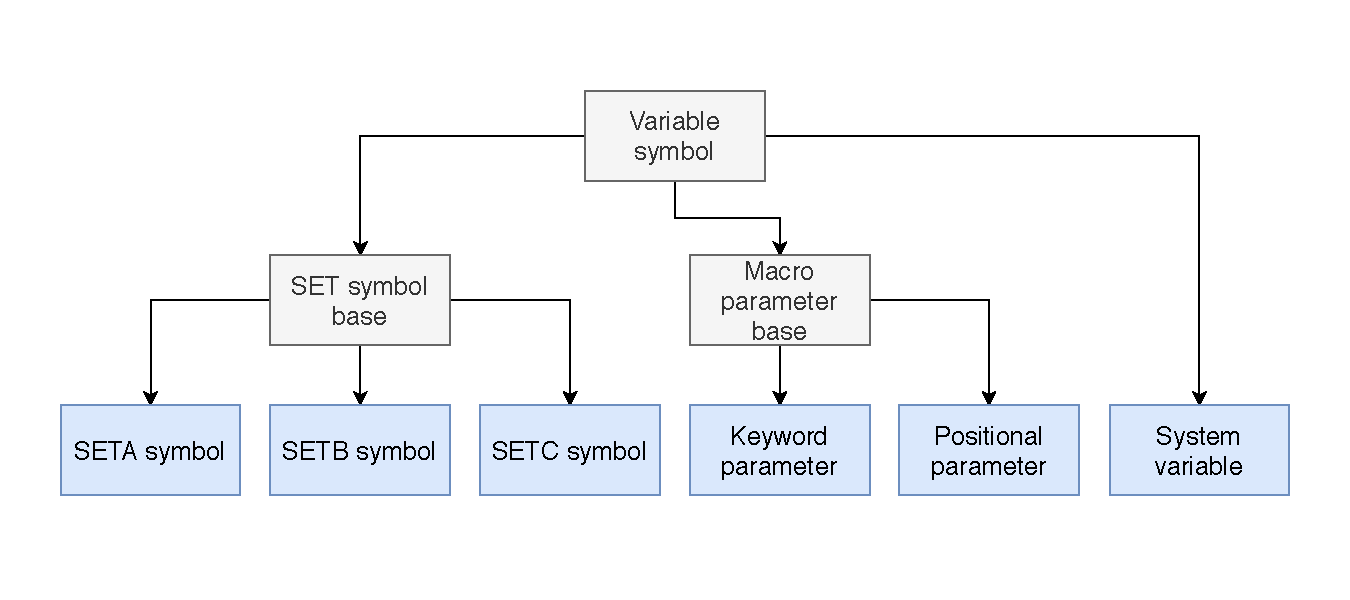
\includegraphics[width=\textwidth]{img/variable_arch}
	\caption{The inheritance of variable symbols.}
	\label{fig06:var}
\end{figure}

\subsection{LSP context}

\subsection{Ordinary assembly context}

The above described structures aimed to describe the high-level part of the language (code generation). As we move closer to the resulting object code of the source file, the describing structures get complicated. Therefore, HLASM context contains object storing just this part of the processing.

\begin{figure}
	\centering
	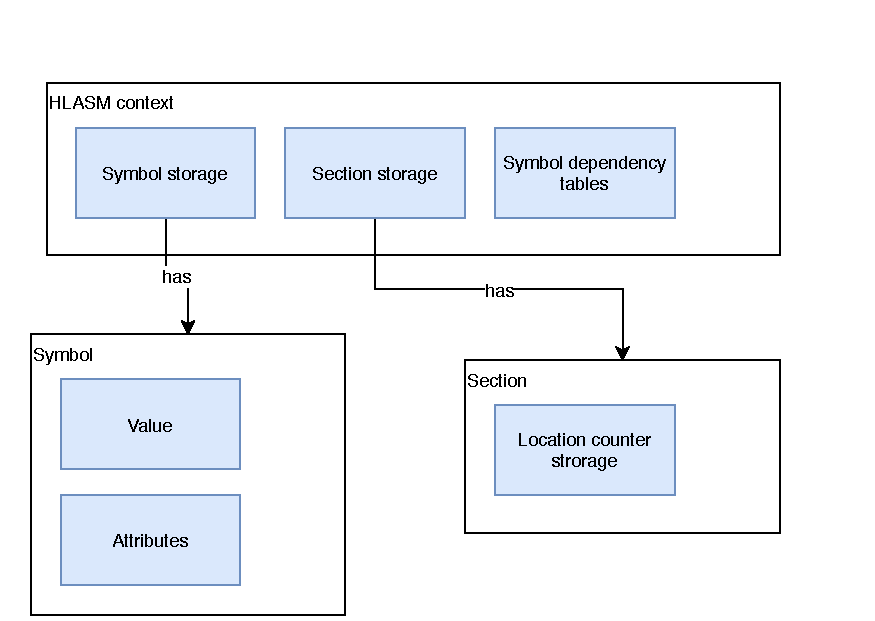
\includegraphics[width=\textwidth / 2]{img/ord_ctx_arch}
	\caption{The composition of Ordinary assembly context}
	\label{fig06:ord_ctx}
\end{figure}

Ordinary assembly context consists of three main components (see \cref{fig06:ord_ctx}):
\begin{enumerate}
	\item \emph{Symbol storage}. Stores ordinary symbols (see \cref{ord_sym}).
	\item \emph{Section storage}. Has notion of all generated sections, each section containing its location counters.
	\item \emph{Symbol dependency tables}. Contains yet unresolved dependencies between symbols prior to the currently processed instruction.
\end{enumerate}

\subsubsection{Symbol}

This class represents HLASM Ordinary symbol (see \cref{ord_sym}). Besides its identifier and location, symbol contains \emph{value} and \emph{attributes} components.

\paragraph*{Value} can be assigned \emph{absolute} or \emph{relocatable} values. With addition to that, it can also be assigned empty value stating that symbol is not yet defined.

\paragraph*{Attributes} structure holds symbol attributes like type, length, scale and integer.

\subsubsection{Section}

Section is a structure representing HLASM section (created by CSECT, DSECT, ...). It contains enumeration \emph{section kind} describing type of the section prior to the used instruction. The structure also holds \emph{location counter storage} with defined location counters.

\subsubsection{Location counter}

This structure contains data and operations for one location counter. The data is stored in helper sub-structure \emph{location counter data}.

\paragraph*{Location counter data} is a structure defining current value of the location counter. It consists of:
\begin{itemize}
	\item \emph{Storage} stating total number of bytes occupied by the location counter.
	\item Vector of \emph{spaces}, block of bytes with yet not known length.
	\item Vector of \emph{storage} between each space.
	\item Currently valid \emph{alignment} (used when data contain spaces).
\end{itemize}

The location counter value is transformable into a relocatable value. It is represented by structure \emph{address}.

\paragraph*{Address} consists of:
\begin{itemize}
	\item Array of \emph{bases}. A base is a beginning of a corresponding section. They serve as points of reference for the address.
	\item Array of \emph{spaces} that are present in the address. 
	\item \emph{Offset} from the bases.
\end{itemize}

The common composition of an address is one base section (as the start of the address) and value of storage (as the offset from it).

The need for the whole array of bases is because addresses from different sections can be arbitrarily added or subtracted. This information is needed as the correct sequence of arithmetic operations can reduce number of bases (even spaces) to zero and create absolute value. This value can be later used in places where a relocatable value would be forbidden.

\paragraph*{Space} is block of bytes with yet not known length. It is created in the active location counter when execution of counter's operation can not be performed due to non previously defined ordinary symbols. See the different kind of spaces and the reason of creation in  the \cref{tab06:space}.

\begin{table}
	\centering
	\begin{tabular}{lr}
		\textbf{Space Kind} &                                          \textbf{Creation} \\ \toprule
		Ordinary            &            when instruction outputs data of unknown length \\
		LOCTR begin         &  when defining more than one location counter in a section \\
		Alignment           &   when current alignment is unknown due to previous spaces \\
		LOCTR set           &     when moving counter's value to the address with spaces \\
		LOCTR max           & when moving counter's value to the next available location \\
		LOCTR unknown       &     when moving counter's value to the yet unknown address \\ \bottomrule
	\end{tabular}
	\caption{Different kinds of spaces and reasons of creation.}
	\label{tab06:space}
\end{table}


When a space length becomes known, all addresses containing the spaces need to be updated (remove the space and append offset). Therefore, space structure contains an array of address listeners. Hence, when an address is assigned a relocatable value that contains the space, the address is added to its array. This serves as an easy point of space resolving.

\vspace{0.5cm}

ORG instruction can arbitrarily move location counter's value forward and backward. With addition to that, ORG can also order location counter to set it's value to the next available value (the lowest untouched address, see \cref{loctr}). Combining this with the possible spaces creation, location counter holds an array of the location counter data to properly set the next available value.

\subsubsection{Symbol dependency tables}
\label{symbol_dependency_tables}
HLASM forbids cyclic symbol definition. This component maintains dependencies between symbols and detects possible cycles.
Let us describe the main components of dependency resolving:

\paragraph*{Dependant} is a structure used in the symbol dependency tables. It encapsulates objects that can be dependent on another. Dependant object can be a \emph{symbol}, \emph{symbol attribute} and \emph{space}.

\paragraph*{Dependable} If an object can contain dependencies, it implements \emph{dependable} interface. The interface has a method to retrieve an structure holding the respective \emph{dependants}. 

\paragraph*{Resolvable} interface adds up to the dependable interface. It is implemented by objects that serve as values assignable to \emph{depednants}. It provides methods to return \emph{symbol value} with help of the dependency solver. 

\paragraph*{Dependency solver} is an interface that can return value of the symbol providing its identifier. It is implemented by Ordinary assembly context.

\vspace{0.5cm}

Having described building blocks, we can move to the symbol dependency tables composition:
\begin{itemize}
	\item \emph{Dependency map}
	\item \emph{Dependency sources map}
	\item \emph{Postponed statements storage}
\end{itemize}

\paragraph*{Dependency map} is the primary storage of dependencies. It has \emph{dependants} as keys and \emph{resolvables} as values. The semantics for pair \emph{(D,R)} is that D is dependent on the dependencies from R. Each time new dependency is added, this map is searched for cycle.

\paragraph*{Dependency sources map} serves as a source objects storage of a resolvable in the dependency map. Hence for the pair \emph{(D,R)} from dependency map, source object of \emph{R} is in the dependency source map under the key \emph{D}. 

The source objects are statements. To be more specific, as one statement can be a source for more distinct resolvables, this source map only stores pointers to the \emph{postponed statements storage}.

\paragraph*{Postponed statements storage} holds statements that are sources of resolvables in dependency map. The reason they are stored is that they can not be checked yet as they contain dependencies. Therefore, they are postponed in the storage until all of the dependencies are resolved. Then they are passed to the respective checker.



